% -------------------------------------------------
\section{Methods and Materials}\label{sec:methods}
% -------------------------------------------------

\subsection{System Architecture}\label{subsec:architecture}
Figure~\ref{fig:architecture} summarises the pipeline.  
A \textbf{Python Ingestor} polls the \textit{AQICN} download endpoint, the \textit{Google Air Quality API}, and the \textit{IQAir API} every ten minutes, saving raw JSON to a versioned MinIO bucket (\texttt{raw-airquality}) for replay and audit purposes\cite{minio,aqicnhist,googleair,iqair}.  
A stateless \textbf{Normalizer} aligns field names, units, and AQI scales before inserting each record into a TimescaleDB hypertable partitioned by \textit{month} and \textit{city}\cite{timescale}.  
Query acceleration relies on concurrent materialised views refreshed with \texttt{REFRESH MATERIALIZED VIEW CONCURRENTLY}\cite{postgsmv}, preventing blocking reads during updates.  
An API layer exposes REST and GraphQL endpoints for different user roles (citizens, researchers, administrators), with Grafana dashboards monitoring ingest lag, API latency, and view-refresh duration in real time\cite{grafana}.  

\begin{figure}[tb]
  \centering
  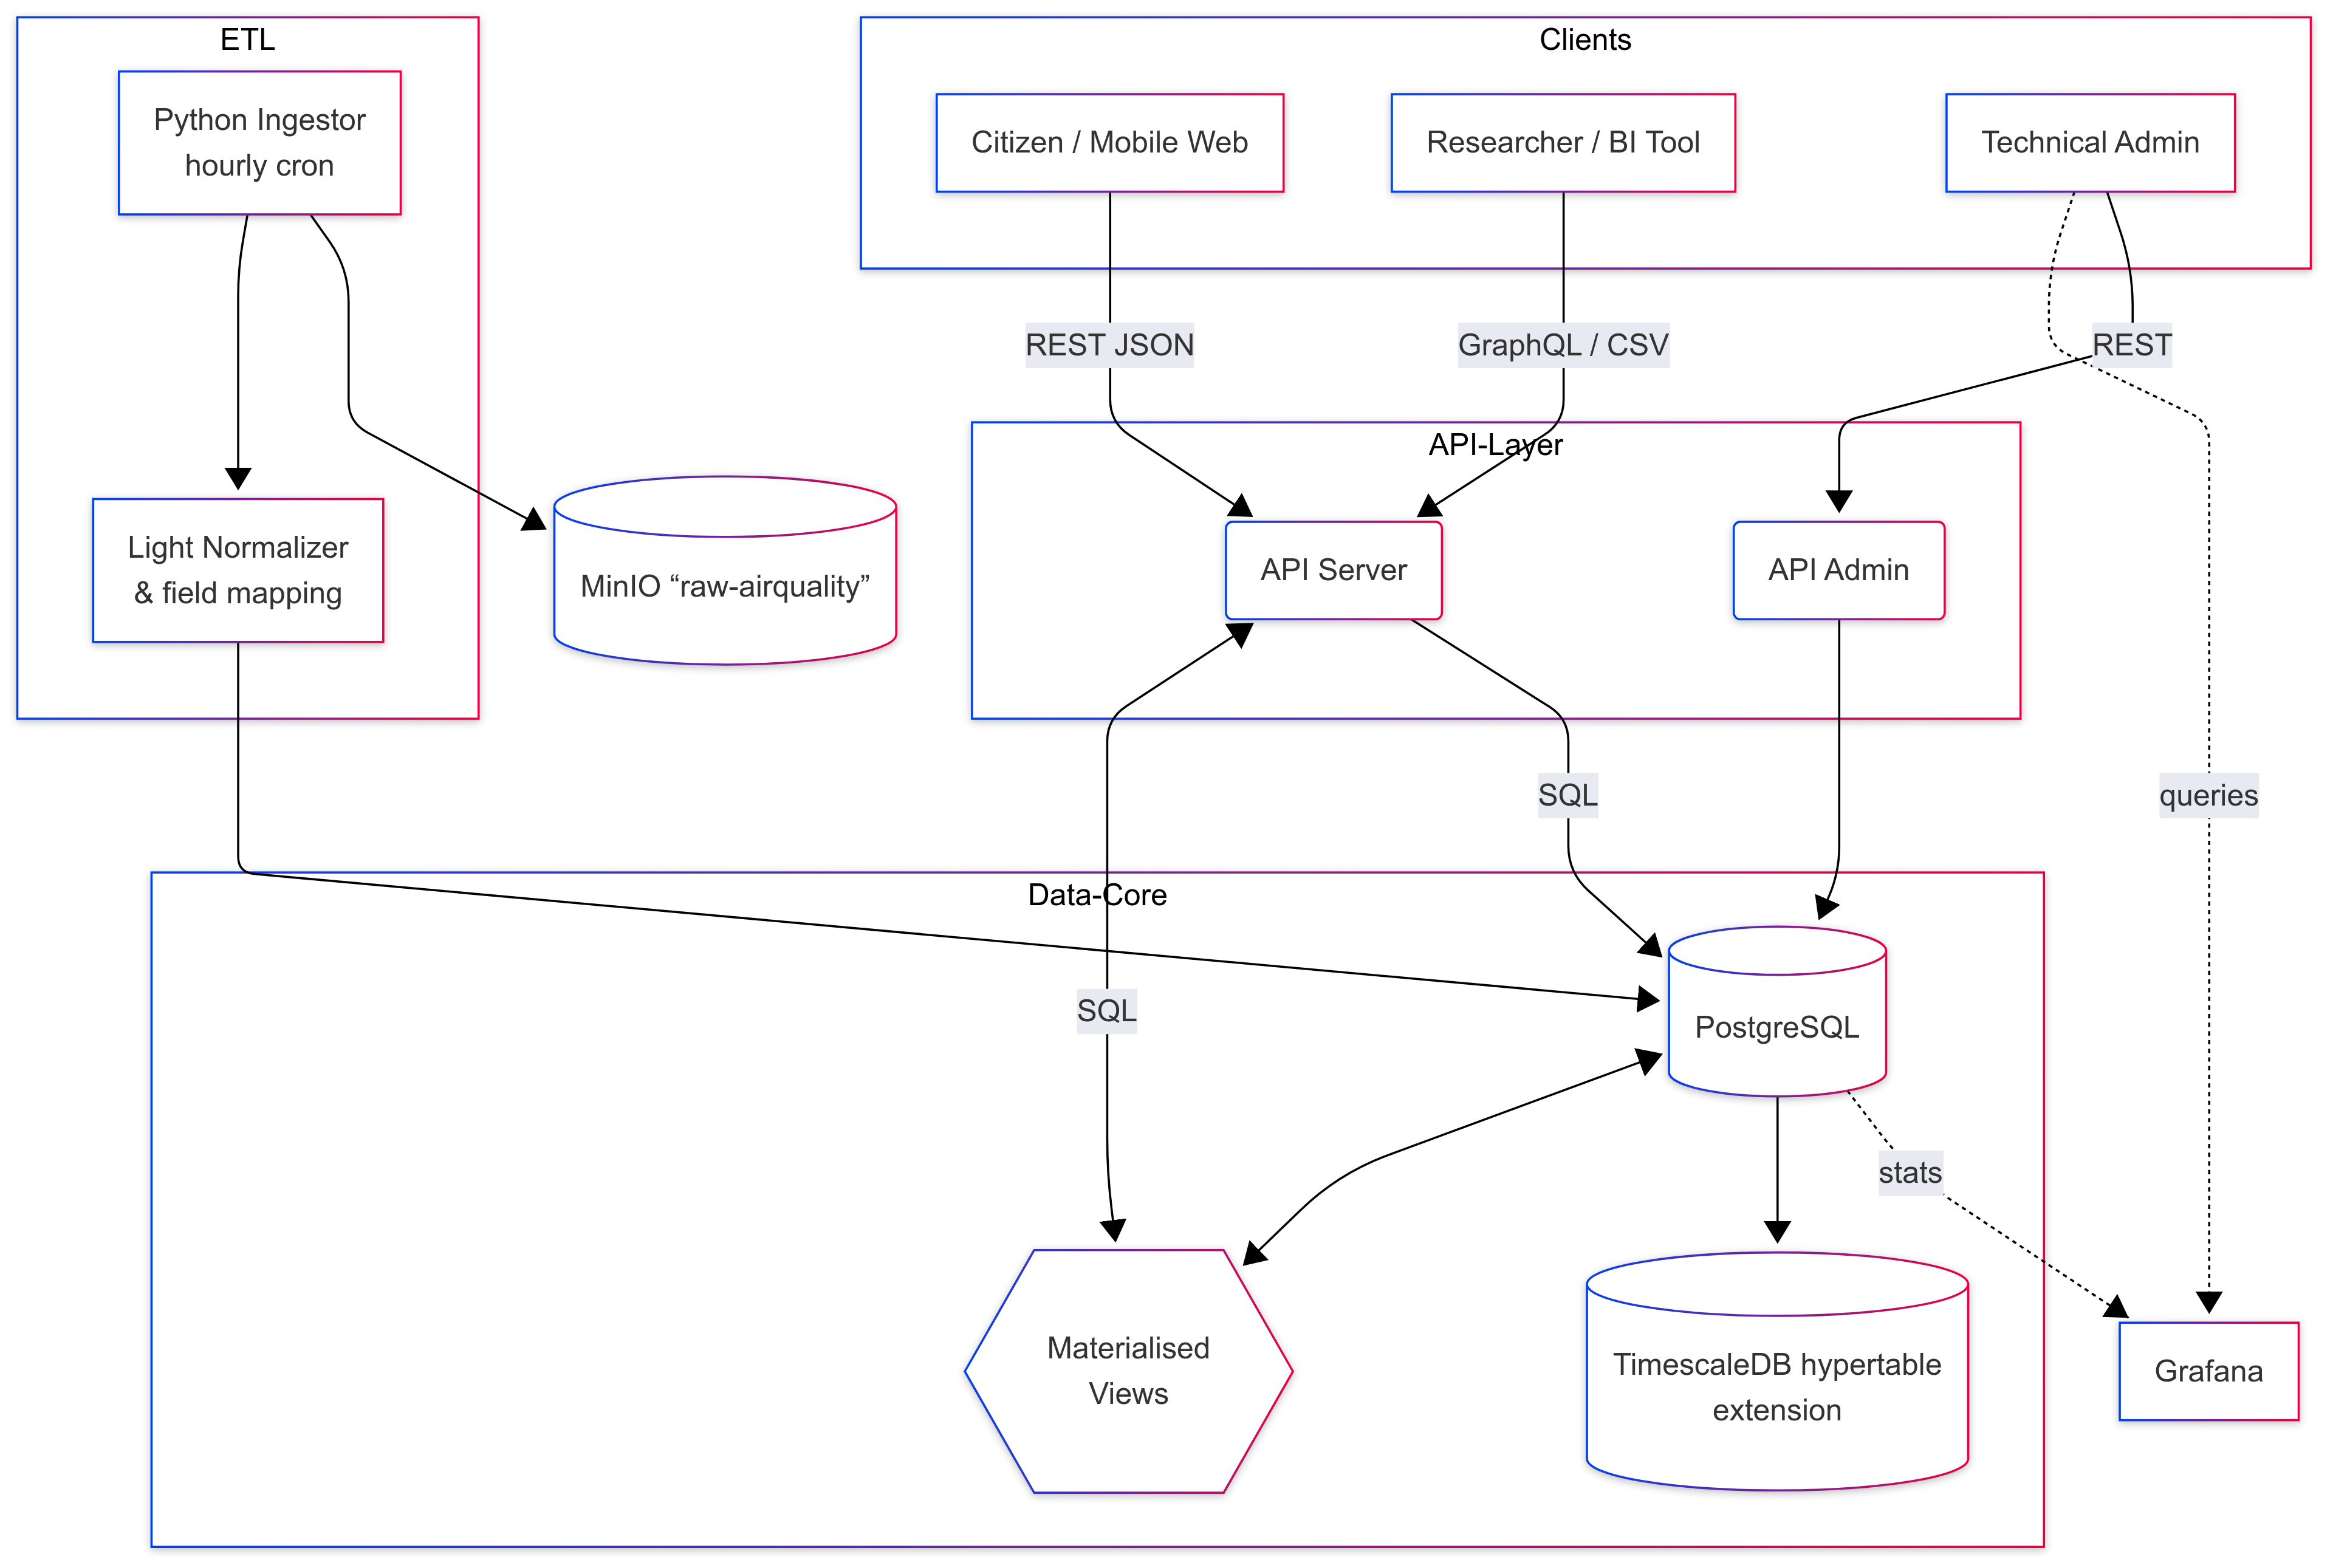
\includegraphics[width=\linewidth]{Pictures/fig1_architecture.png}
  \caption{End-to-end architecture (planned).}
  \label{fig:architecture}
\end{figure}

\subsection{Data Modelling and Partitioning}\label{subsec:partitioning}
The relational schema comprises thirteen entities organized into three logical layers: \textit{Geospatial} (Station, AirQualityReading, Pollutant, MapRegion), \textit{Customer} (User, Role, Permission, RolePermission, DashboardConfig), and \textit{Recommendation Engine} (Alert, Recommendation, ProductRecommendation, Report).  
The primary table \texttt{airquality\_reading} is implemented as a monthly-partitioned TimescaleDB hypertable whose chunks are expected to contain \(\approx\!2.5\;\mathrm{M}\) rows per month for Bogotá under current ingestion rates\cite{timescale}.  
Temporal and geographic partitioning enables efficient pruning of irrelevant data during time-localized and city-specific queries, reducing index scan sizes and improving concurrent access performance.  
Foreign keys enforce referential integrity between stations, pollutants, users, and recommendations as defined in the complete ER diagram available in the project repository.

\subsection{Personalised Recommendation Engine}\label{subsec:reco}
The recommendation engine implements functional requirements FR8–FR11 through a multi-stage pipeline.  
First, each new air quality observation is classified into EPA AQI bands (Good 0–50, Moderate 51–100, Unhealthy for Sensitive Groups 101–150, Unhealthy 151–200, Very Unhealthy 201–300, Hazardous >300)\cite{epaaqi}.  
The AQI category is then combined with user metadata—location preferences, activity type (e.g., outdoor exercise, commuting), and health risk profile—to generate personalized health advice aligned with WHO guidelines\cite{whoaq}.  
When \(\text{AQI}\ge151\) (Unhealthy threshold), the system optionally appends suggestions for certified protective products (e.g., N95 masks, air purifiers) retrieved from a curated \texttt{product\_recommendation} catalog linked to active recommendations.  
Users can configure custom alert thresholds per pollutant type (PM$_{2.5}$, PM$_{10}$, O$_3$, NO$_2$, SO$_2$, CO) with delivery via email or push notification as specified in user story US9.  
To prevent notification fatigue during stable pollution periods, recommendations are cached in-memory (LRU eviction policy, 3-hour TTL) and refreshed only when AQI changes by more than one category or user location shifts beyond a 2~km radius.

\subsection{Concurrency Control and Performance Optimization}\label{subsec:concurrency}
The platform addresses several concurrency scenarios inherent to multi-user, real-time systems.  
To prevent write conflicts during simultaneous API ingestion, each data source writes to the database within independent transactions protected by unique constraints on (\texttt{station\_id}, \texttt{pollutant\_id}, \texttt{datetime}) tuples.  
User-editable tables (\texttt{alert}, \texttt{dashboard\_config}) implement optimistic concurrency control using \texttt{last\_updated} timestamp fields; conflicting updates are detected before commit and trigger a retry mechanism.  
For high-contention scenarios such as concurrent alert modifications from multiple devices, row-level locks (\texttt{SELECT ... FOR UPDATE}) ensure atomic read-modify-write sequences.  
The concurrent materialized view refresh strategy eliminates the risk of dirty reads during dashboard queries, allowing users to access consistent snapshots even while aggregations are being recomputed.  
Future architectural iterations will explore read replicas for dashboard traffic separation and message queues (Kafka or RabbitMQ) for fully asynchronous ingestion pipelines, as outlined in performance improvement strategies.

\subsection{Planned Experimental Environment}\label{subsec:experiment}
Because the platform is still under active construction, we specify the \textit{target} test bench so reviewers can reproduce forthcoming benchmarks:

\begin{itemize}
  \item \textbf{Dataset.} Historical CSV archives published by AQICN starting in 2015\cite{aqicnhist}.  
        Phase 1 will ingest three years (2022–2024) of Bogotá air quality data; phase 2 may expand to 2018–2024 if storage capacity and ingestion performance targets are met.
        Each CSV row follows the schema \texttt{Date, Country, City, Specie, count, min, max, median, variance}.
  \item \textbf{Hardware (planned).} Primary database node: 4 vCPU, 16 GB RAM, NVMe storage; object storage layer (MinIO) with sufficient capacity for raw JSON archives.
  \item \textbf{Software versions (expected).} PostgreSQL 17.1, TimescaleDB 2.14, MinIO (latest stable release), Grafana 11, Python 3.12.
  \item \textbf{Load test design.} Apache JMeter scripts will simulate 1000 concurrent users accessing dashboards and generating reports, each issuing approximately 5 REST/GraphQL requests per second over a 10-minute test window\cite{jmeter}.  
        Performance metrics (query latency, throughput, CPU utilization) will be collected via Prometheus exporters and \texttt{pg\_stat\_statements}, with real-time visualization in Grafana\cite{grafana}.
  \item \textbf{Target metrics.} The system aims to satisfy NFR1 (queries over 1M records in <2s at p95), NFR4 (report generation in <10s), NFR5 (recommendation updates every 10 minutes), and NFR6 (dashboard load times <2s at p95).
\end{itemize}